\newpage
\appendix
\section*{Appendix}
\addcontentsline{toc}{section}{Appendix}
\renewcommand{\thesubsection}{\Roman{subsection}}
\subsection{Code}
\label{appendix:code}
\begin{figure}[H]
    \centering
    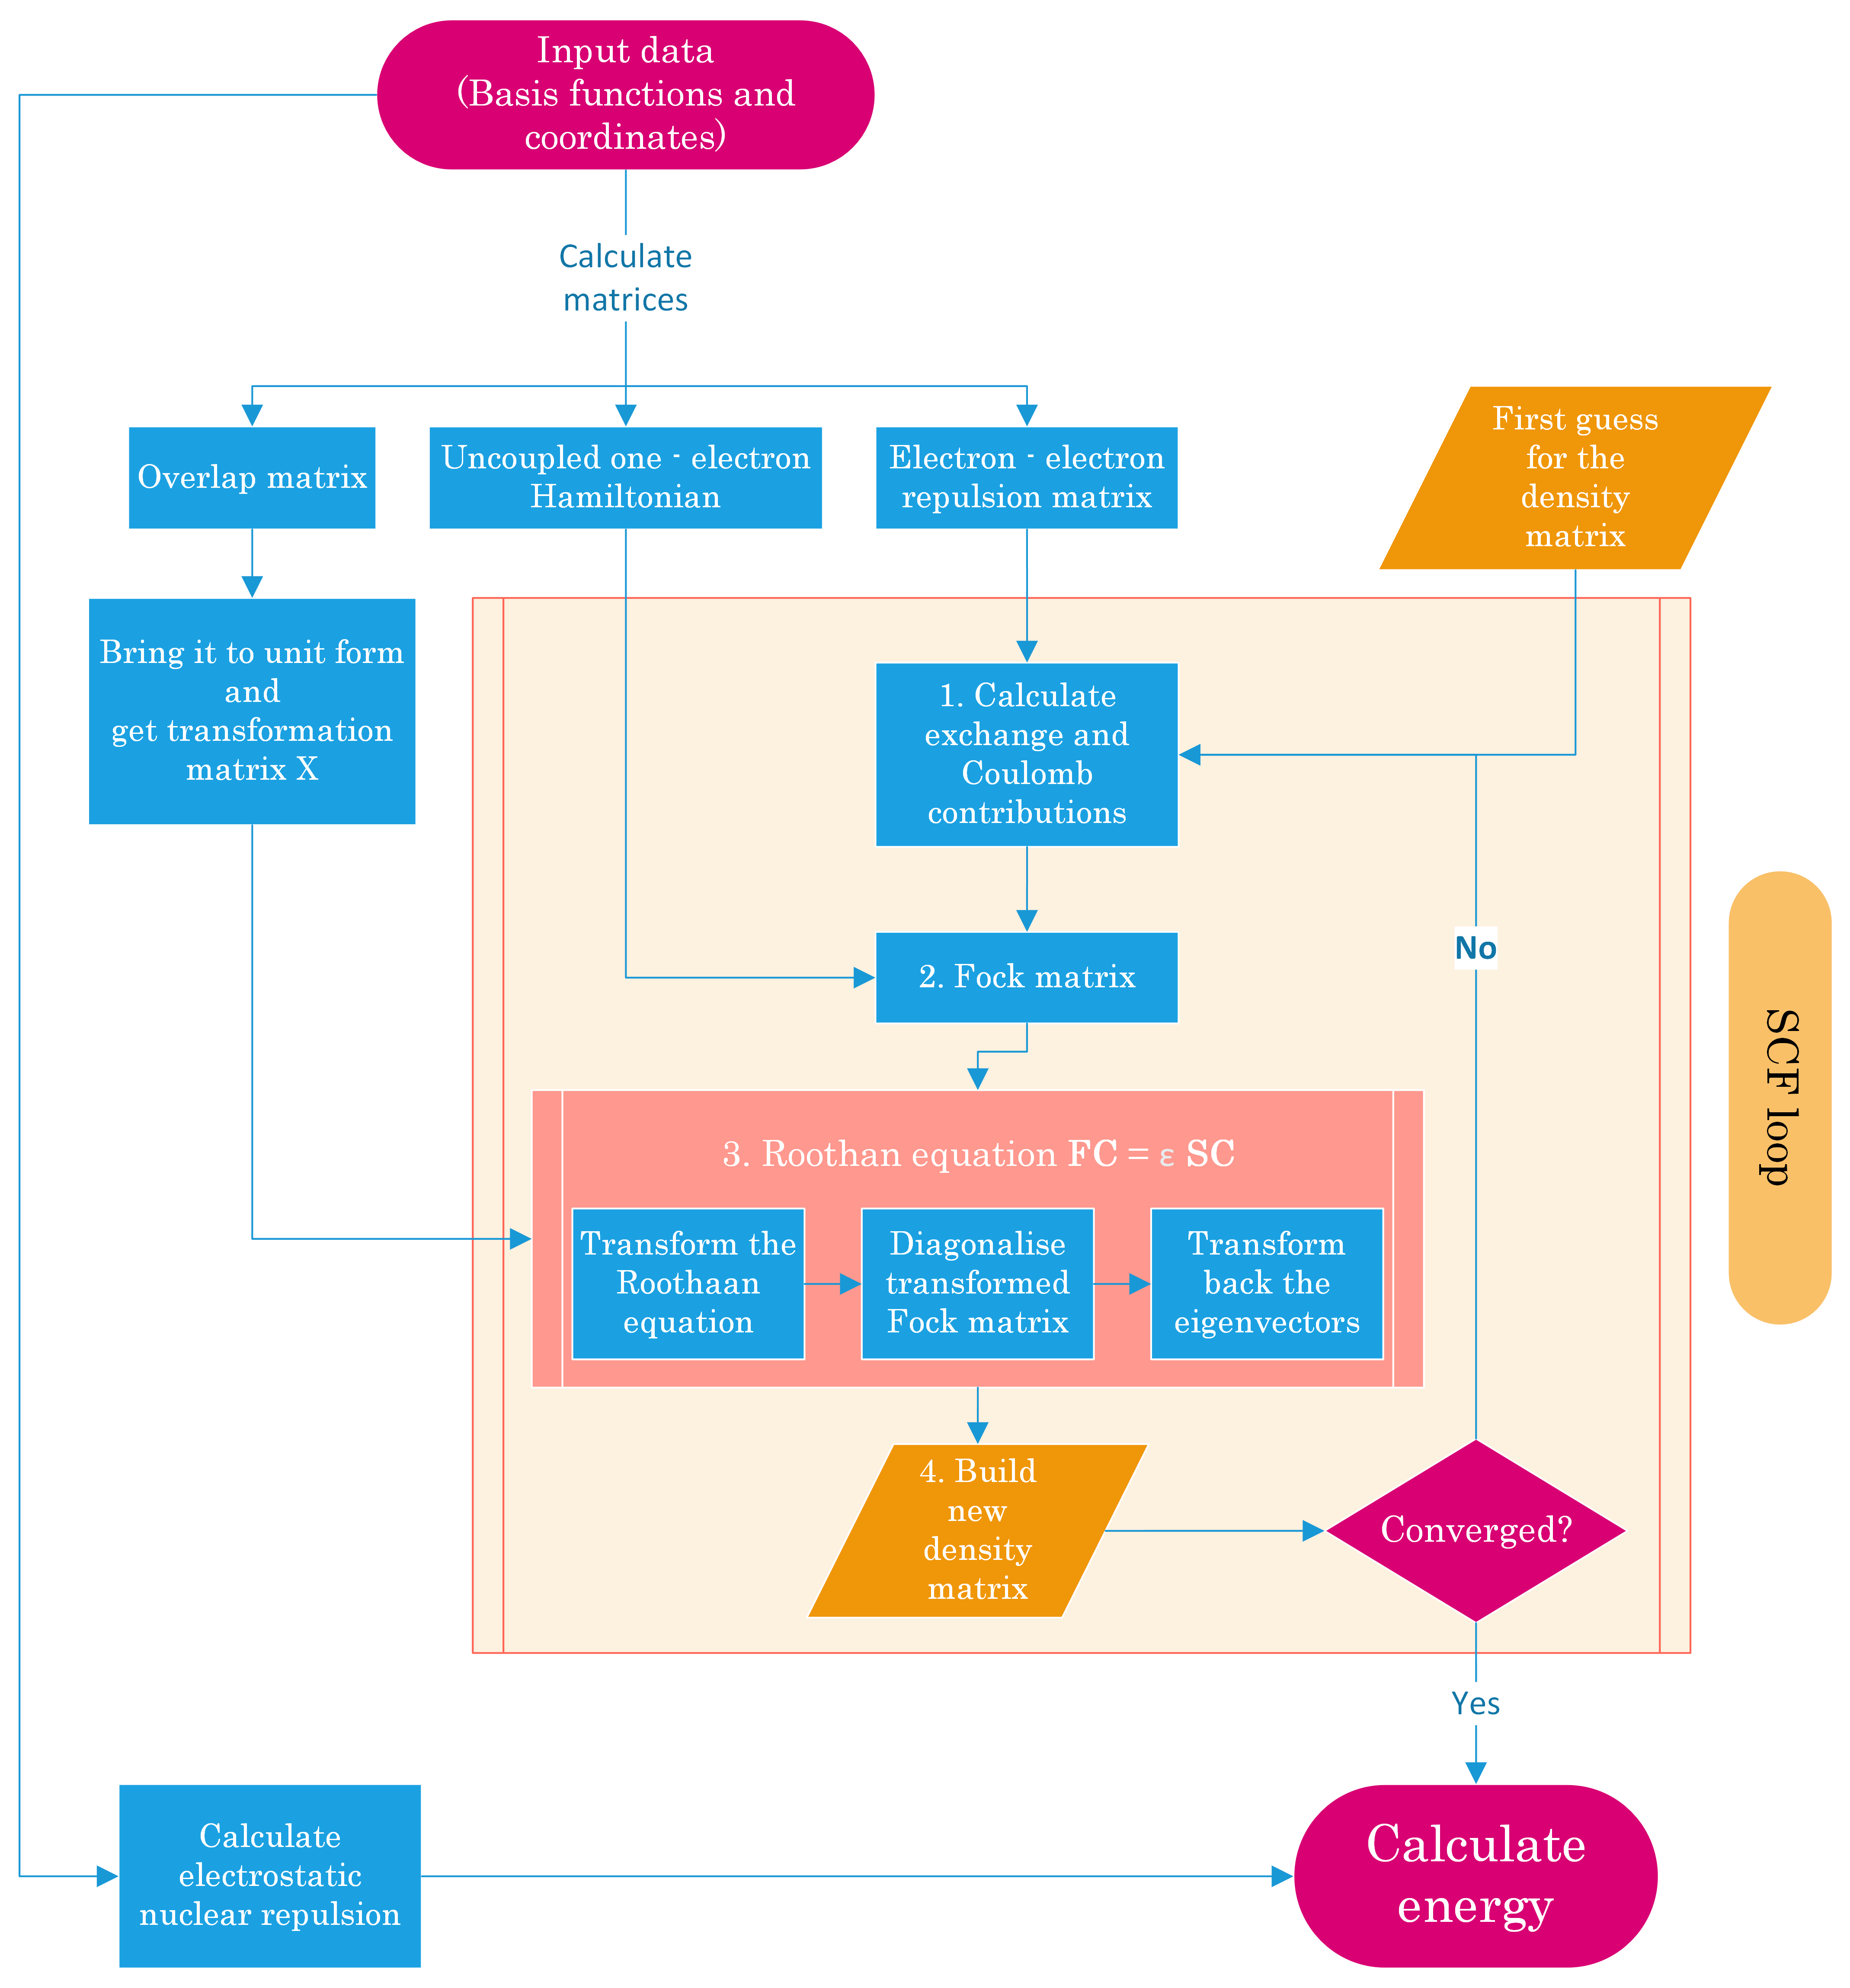
\includegraphics[width = \textwidth]{HF_flowchart}
    \caption{Flow chart of a Hartree-Fock program.}
    \label{fig:flowchart}
\end{figure}
\subsection{On the energy expression derivation}\label{appendix:energies}
The expression of the energy can be obtained, as usual, by calculating the expectation value of the Hamiltonian. Assuming the use of a single Slater determinant and within the frame of the Born-Oppenheimer approximation, the Hamiltonian (\ref{eq:hart1}) has the form
\begin{align}\label{eq:hamiltonian_derivation}
    &H=\sum_i^N h(i)+\frac{1}{2}\sum_{i,j;i\neq j}^Ng(i,j),\; \; \mathrm{where}\\
    &h(i)=-\frac{1}{2}\nabla_i^2-
\sum_{n=1}^K \frac{Z_n}{\left|\mathbf{r}_i -\mathbf{R}_n\right|}\; \; \mathrm{and}\nonumber\\
    &g(i,j) = \frac{1}{\left|\mathbf{r}_i -\mathbf{r}_j\right|}.\nonumber
\end{align}
By taking $\psi$ to be the Slater determinant of a Hartree product, and introducing the notation:
\begin{equation}
    \mel{\psi_k \psi_l}{g}{\psi_m\psi_n} = \int{d\mathbf{x_1}d\mathbf{x_2}\psi_k^*(\mathbf{x_1})\psi_l^*(\mathbf{x_2})\frac{1}{\left|\mathbf{r}_i -\mathbf{r}_j\right|}\psi_m(\mathbf{x_1})\psi_n(\mathbf{x_2})}
\end{equation}
one can get the expectation value of the energy as
\begin{equation}
    E = \sum_k^N\mel{\psi_k}{h}{\psi_k}+\frac{1}{2}\sum_{k,l}^N\left(\mel{\psi_k \psi_l}{g}{\psi_k\psi_l}-\mel{\psi_k \psi_l}{g}{\psi_l\psi_k}\right).
    \label{eq:unsimple_energy}
\end{equation}
Moreover, by defining the Coulomb and exchange operators respectively:
\begin{align}
    J=\sum_k^NJ_k& : J_k(\mathbf{x})\psi(\mathbf{x})=\int{d\mathbf{x}'\psi_k^*(\mathbf{x})' \frac{1}{\left|\mathbf{r}_i -\mathbf{r}_j\right|}\psi_k(\mathbf{x}')\psi(\mathbf{x})}\\
    K=\sum_k^NK_k& : K_k(\mathbf{x})\psi(\mathbf{x})=\int{d\mathbf{x}'\psi_k^*(\mathbf{x})'\frac{1}{\left|\mathbf{r}_i -\mathbf{r}_j\right|} \psi(\mathbf{x}')\psi_k(\mathbf{x})}
\end{align}
the energy functional has the simpler form
\begin{equation}
    E=\sum_k^N\ev{\psi_k \left| h + \frac{1}{2}(J-K) \right| \psi_k}
    \label{eq:energy_hJK}
\end{equation}
Now, by defining the Fock operator
\begin{equation}
    \mathcal{F}=h+J-K
\end{equation}
which satisfies the eigenvalue equation
\begin{equation}
    \mathcal{F}\psi_k   = \varepsilon_k\psi_k,
\end{equation}
the relationship between the eigenvalues $\varepsilon_k$ and the energy (\ref{eq:energy_hJK}) can be obtained as follows:
\begin{align}
    E &= \sum_k^N\left[\ev{\psi_k \left| h\right| \psi_k}+\ev{\psi_k \left|\frac{1}{2}(J-K) \right| \psi_k}\right]=\nonumber\\&=\sum_k^N\left[\varepsilon_k-\ev{\psi_k \left|\frac{1}{2}(J-K) \right| \psi_k} \right]=\sum_k^N\left[\varepsilon_k+\mel{\psi_k}{h}{\psi_k} \right]-E\Leftrightarrow\nonumber\\&\Leftrightarrow E=\frac{1}{2}\sum_k^N\left[\varepsilon_k+\mel{\psi_k}{h}{\psi_k} \right]
    \label{eq:energyobtained}
\end{align}
which can be identified as the expression presented in the work (\ref{eq:energies_heps}).\\\\
After redefining the Fock, Coulomb and exchange operators for the spatial orbitals such that the Fock equation reads $F = h+2J-K$  ---see equation (\ref{eq:new_HF})---, the energy is given by an analogous expression to (\ref{eq:energy_hJK}):
\begin{equation}
    E = 2\sum_k^{N/2}\mel{\phi_k}{h}{\phi_k}+\sum_k^{N/2}\left(2\mel{\phi_k}{J}{\phi_k}-\mel{\phi_k}{K}{\phi_k}\right)
\end{equation}
As it is presented in the work, from now on it will be assumed that sums over $k$ extend to all different spatial orbitals (this is, half of the total number of orbitals, $N/2$).

Now, by introducing the parametrisation 
\begin{equation}
    \phi_k=\sum_{q}^MC_{qk}\chi_q(\mathbf{r})
    \label{eq:parametrisation}
\end{equation}
the energy can be written as
\begin{equation}
    E = \sum_{p,q}^MP_{pq} h_{pq} + \frac{1}{2}\sum_{p,q,r,s}^M P_{pq}P_{rs}\left[\mel{pr}{g}{qs}-\frac{1}{2}\mel{pr}{g}{sq}\right]
\end{equation}
where $\mathbf{P}$ is the density matrix defined in (\ref{eq:density_matrix}) and $\mel{pr}{g}{qs}$ represent a two-electron integral using the notation presented in (\ref{eq:g_matrix}).

Moreover, an equivalent expression dependent on the Fock levels ---the eigenvalues $\varepsilon_k$ of the new Fock operator $F$--- can be found:
\begin{align}
    \sum_k \varepsilon_k &= \sum_k\left[\mel{\phi_k}{h}{\phi_k}+2\mel{\phi_k}{J}{\phi_k}-\mel{\phi_k}{K}{\phi_k}\right]\nonumber\\
    &=\sum_k\mel{\phi_k}{h}{\phi_k} + E - 2\sum_k\mel{\phi_k}{h}{\phi_k} = E - \sum_k\mel{\phi_k}{h}{\phi_k}\Leftrightarrow\nonumber\\
    &\Leftrightarrow E = \sum_k \left[\varepsilon_k + \mel{\phi_k}{h}{\phi_k}\right]
\end{align}
which, again, by introducing the parametrisation (\ref{eq:parametrisation}) and the density matrix,
\begin{equation}
    E = \frac{1}{2}\sum_{p,q}^MP_{pq} h_{pq}+\sum_k \varepsilon_k
\end{equation}
It should be remembered that the total energy of the system shall include as well the internuclear repulsion energy for the given configuration.